% =================================================================================================
% File:			dia_seq_server.tex
% Description:	Definisce la sezione relativa al capitolo relativo ai diagrammi di sequenza tra i componenti del server
% Created:		2015-05-22
% Author:		Faccin Nicola
% Email:		faccin.nicola@mashup-unipd.it
% =================================================================================================
% Modification History:
% Version		Modifier Date		Change											Author
% 0.0.1 		2015-05-22 			creato scheletro doc							Nicola Faccin
% =================================================================================================
%

% CONTENUTO DEL CAPITOLO

\subsection{Server} % (fold)
\label{ssub:diagrammi_di_sequenza_server}
Quelli che seguono sono i diagrammi di sequenza che rappresentano le più rilevanti interazioni tra i vali moduli presenti nel livello server. Per quanto riguarda il client, fare riferimento alla sezione \ref{ssub:diagrammi_di_sequenza_client}.

    \subsubsection{Cron task} % (fold)
    \label{ssub:cron_task}
    Il seguente diagramma descrive il processo di avvio dell'aggiornamento dei dati grezzi relativi ad ogni Recipe presente nel sistema. Tale sequenza è attivata a cadenza regolare tramite le funzionalità di \textit{task scheduling} offerte da Google App Engine. Per semplicità, è stato descritto in dettaglio esclusivamente l'aggiornamento dei dati relativi a Facebook, indicando solamente i metodi principali per i restanti social network. \newline

    \begin{figure}[!htbp]
		\centering
			\centerline{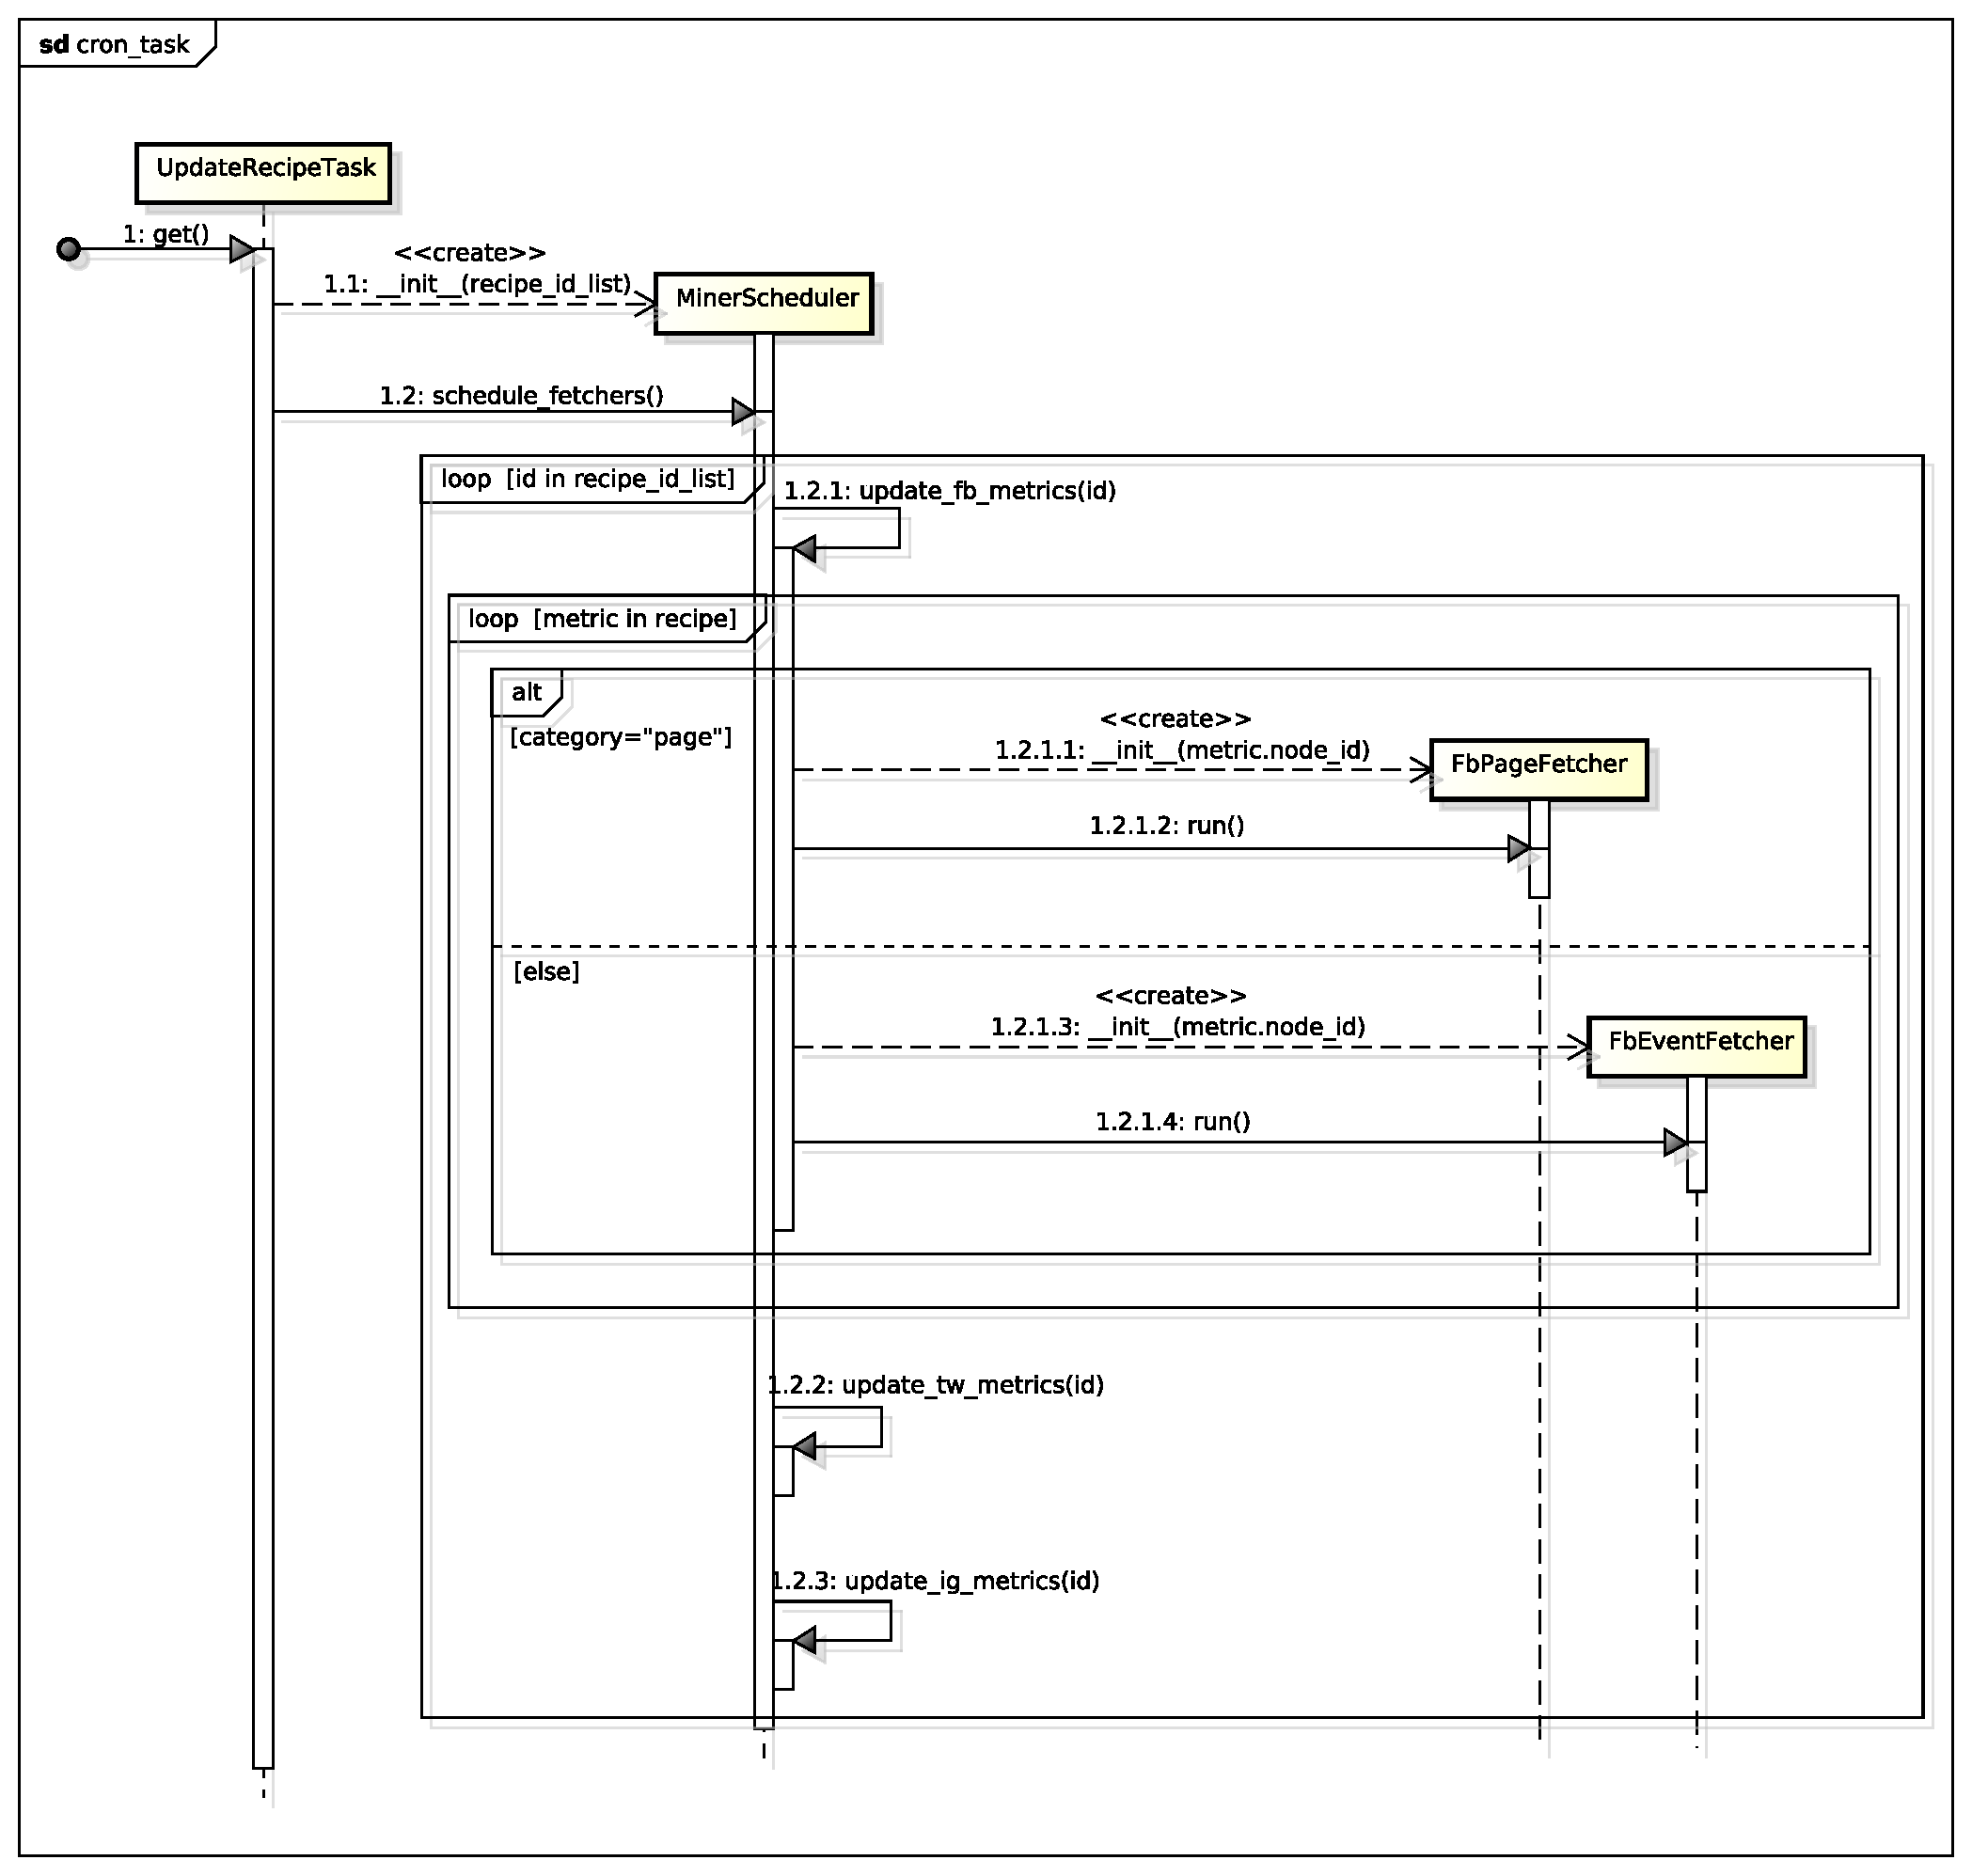
\includegraphics[scale=0.4]{./images/sequence_diagram/cron_task.pdf}}
		\caption{Diagramma di sequenza - Cron task}
	\end{figure}

    \begin{itemize}
        \item \textbf{UpdateRecipeTask}: classe implementata secondo gli standard di Google App Engine, definisce il metodo statico \texttt{get()} attivato ad ogni avvio del componente Cron di Google. \texttt{UpdateRecipeTask} istanzia la classe \texttt{MinerManager} invocando il metodo \texttt{schedule\_fetchers(recipe\_id\_list)} per effettuare l'aggiornamento dei dati grezzi;
        \item \textbf{MinerScheduler}: definisce il metodo \texttt{schedule\_fetchers(recipe\_id\_list)} che cicla la lista di id delle Recipe scadute invocando per ognuna il metodo \texttt{update\_fb\_metrics(id)} per ogni metrica Facebook contenuta nella Recipe in questione. Tale metodo avvia un fetcher differente a seconda del tipo di metrica ricavata. Tale procedimento avviene sequenzialmente anche per gli altri social tramite i metodi \texttt{update\_tw\_metrics(id)} e \texttt{update\_ig\_metrics(id)};
        \item \textbf{FbPageFetcher}: classe che viene istanziata ed avviata tramite il metodo \texttt{run()} per avviare l'aggiornamento dei dati relativi ad una pagina Facebook;
        \item \textbf{FbEventFetcher}: classe che viene istanziata ed avviata tramite il metodo \texttt{run()} per avviare l'aggiornamento dei dati relativi ad un evento Facebook.
    \end{itemize}


	\subsubsection{Miner Facebook} % (fold)
    \label{ssub:miner_facebook}
    Il diagramma alla figura~\ref{fig:miner_facebook} descrive l'aggiornamento dei dati, relativi ad una metrica che descrive una pagina di Facebook, a seguito della chiamata del cron che richiede l'aggiornamento della Recipe a cui la metrica appartiene. Tale sequenza verrà attivata ogni qualvolta una metrica che descrive una pagina di Facebook dovrà essere aggiornata. \newline

    \begin{figure}[!htbp]
		\centering
			\centerline{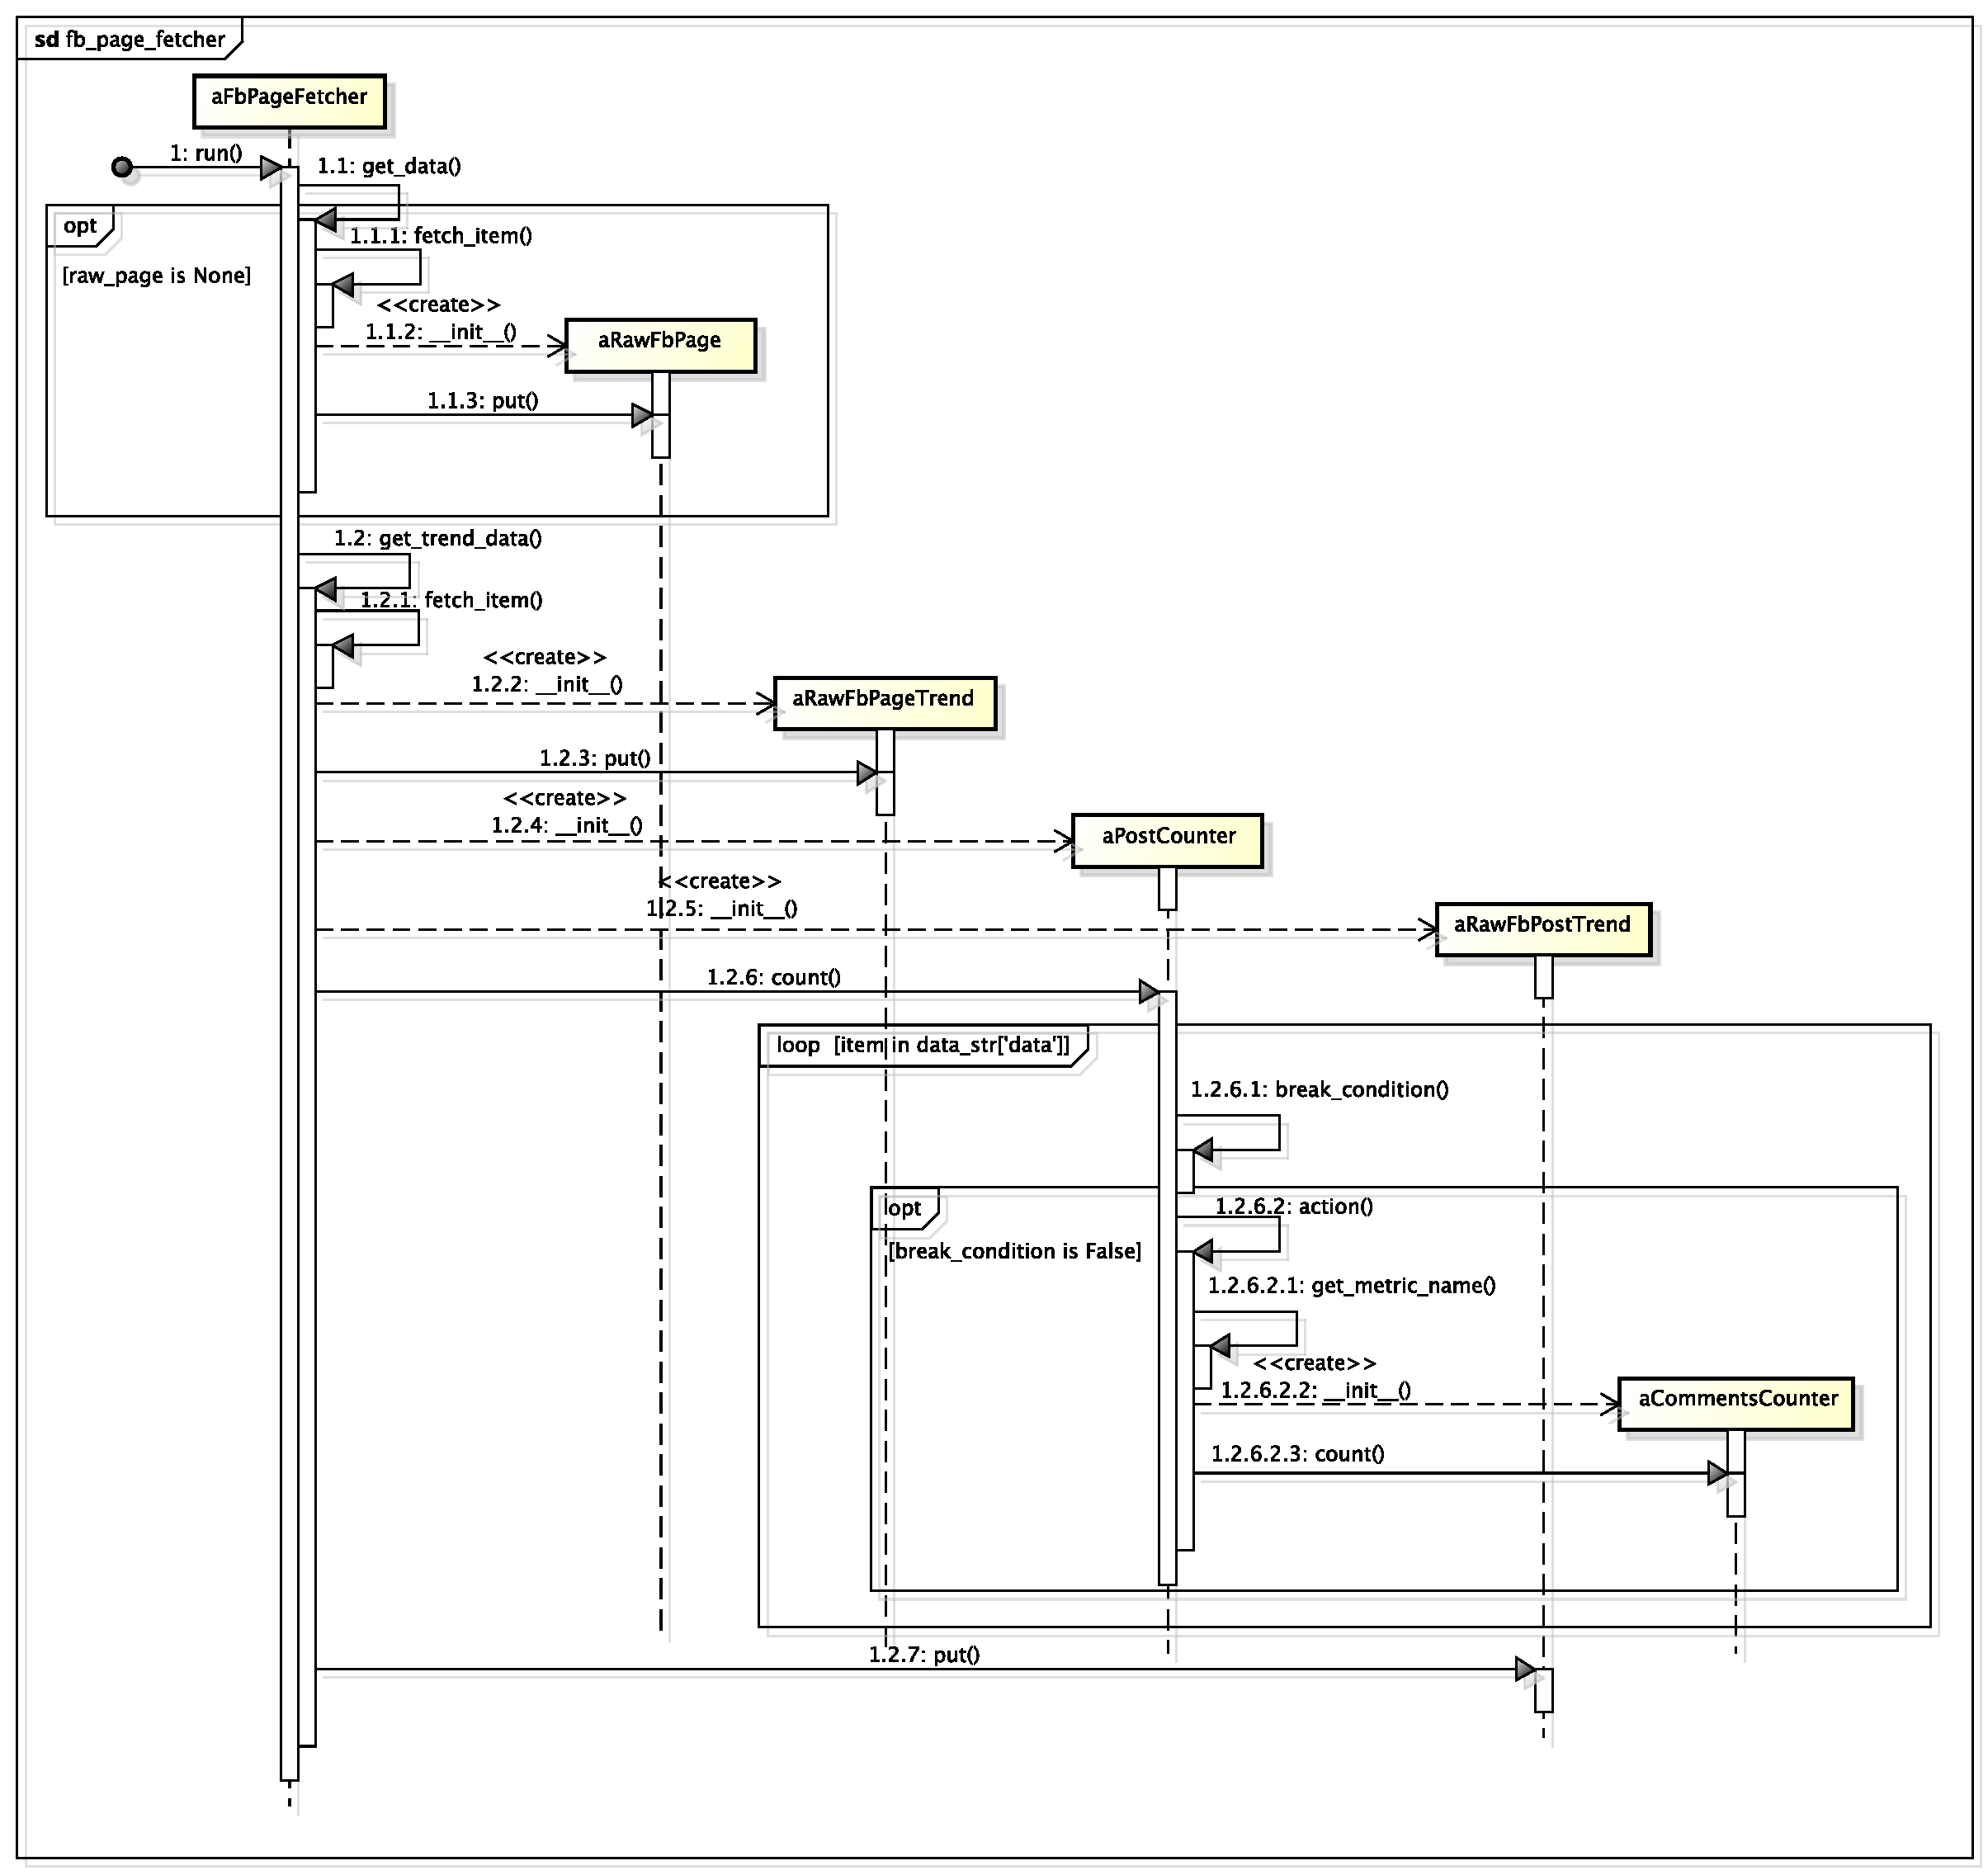
\includegraphics[scale=0.4]{./images/sequence_diagram/fb_page_fetcher.pdf}}
		\caption{Diagramma di sequenza - Miner Facebook}
    \label{fig:miner_facebook}
	\end{figure}


    \begin{itemize}
        \item \textbf{FbPageFetcher}: classe richiamata dalla classe \texttt{MinerScheduler} e contenente i metodi \texttt{get\_data()} e \texttt{get\_trend\_data()}. Il primo metodo si occupa di recuperare i dati statici di una pagina Facebook se non ancora presente nel database; il secondo metodo si occupa di recuperare i dati dinamici della pagina;
        \item \textbf{RawFbPage}: classe utilizzata dal metodo \texttt{get\_data()} della classe \texttt{FbPageFetcher} per salvare i dati statici di una pagina Facebook tramite il metodo \texttt{put()};
        \item \textbf{RawFbPageTrend}: classe utilizzata dal metodo \texttt{get\_trend\_data()} della classe \texttt{FbPageFetcher} per salvare i dati dinamici di una pagina Facebook tramite il metodo \texttt{put};
        \item \textbf{PostCounter}: classe utilizzata dal metodo \texttt{get\_trend\_data()} della classe \texttt{FbPageFetcher} per effettuare il conteggio dei post di una pagina nell'arco di tre giorni e per calcolarsi i vari trend relativi ai post;
        \item \textbf{CommentCounter}: classe utilizzata dal metodo \texttt{action()} della classe \texttt{PostCounter} per effettuare il conteggio dei commenti in un post tramite il metodo \texttt{count()};
        \item \textbf{RawFbPostTrend}: classe utilizzata dal metodo \texttt{get\_trend\_data()} della classe \texttt{FbPageFetcher} per salvare i dati dinamici relativi ai post all'interno di una pagina Facebook tramite il metodo \texttt{put()}.
    \end{itemize}


	\subsubsection{Login API} % (fold)
    \label{ssub:login_api}
    Il diagramma nella figura~\ref{fig:login_api} descrive il funzionamento del servizio REST di autenticazione offerto dal sistema. Il client tramite il metodo \texttt{login()} della classe \texttt{DataManagerService} utilizza il servizio REST di autenticazione definito nella classe \texttt{OAuthApi}. \newline

    \begin{figure}[!htbp]
		\centering
			\centerline{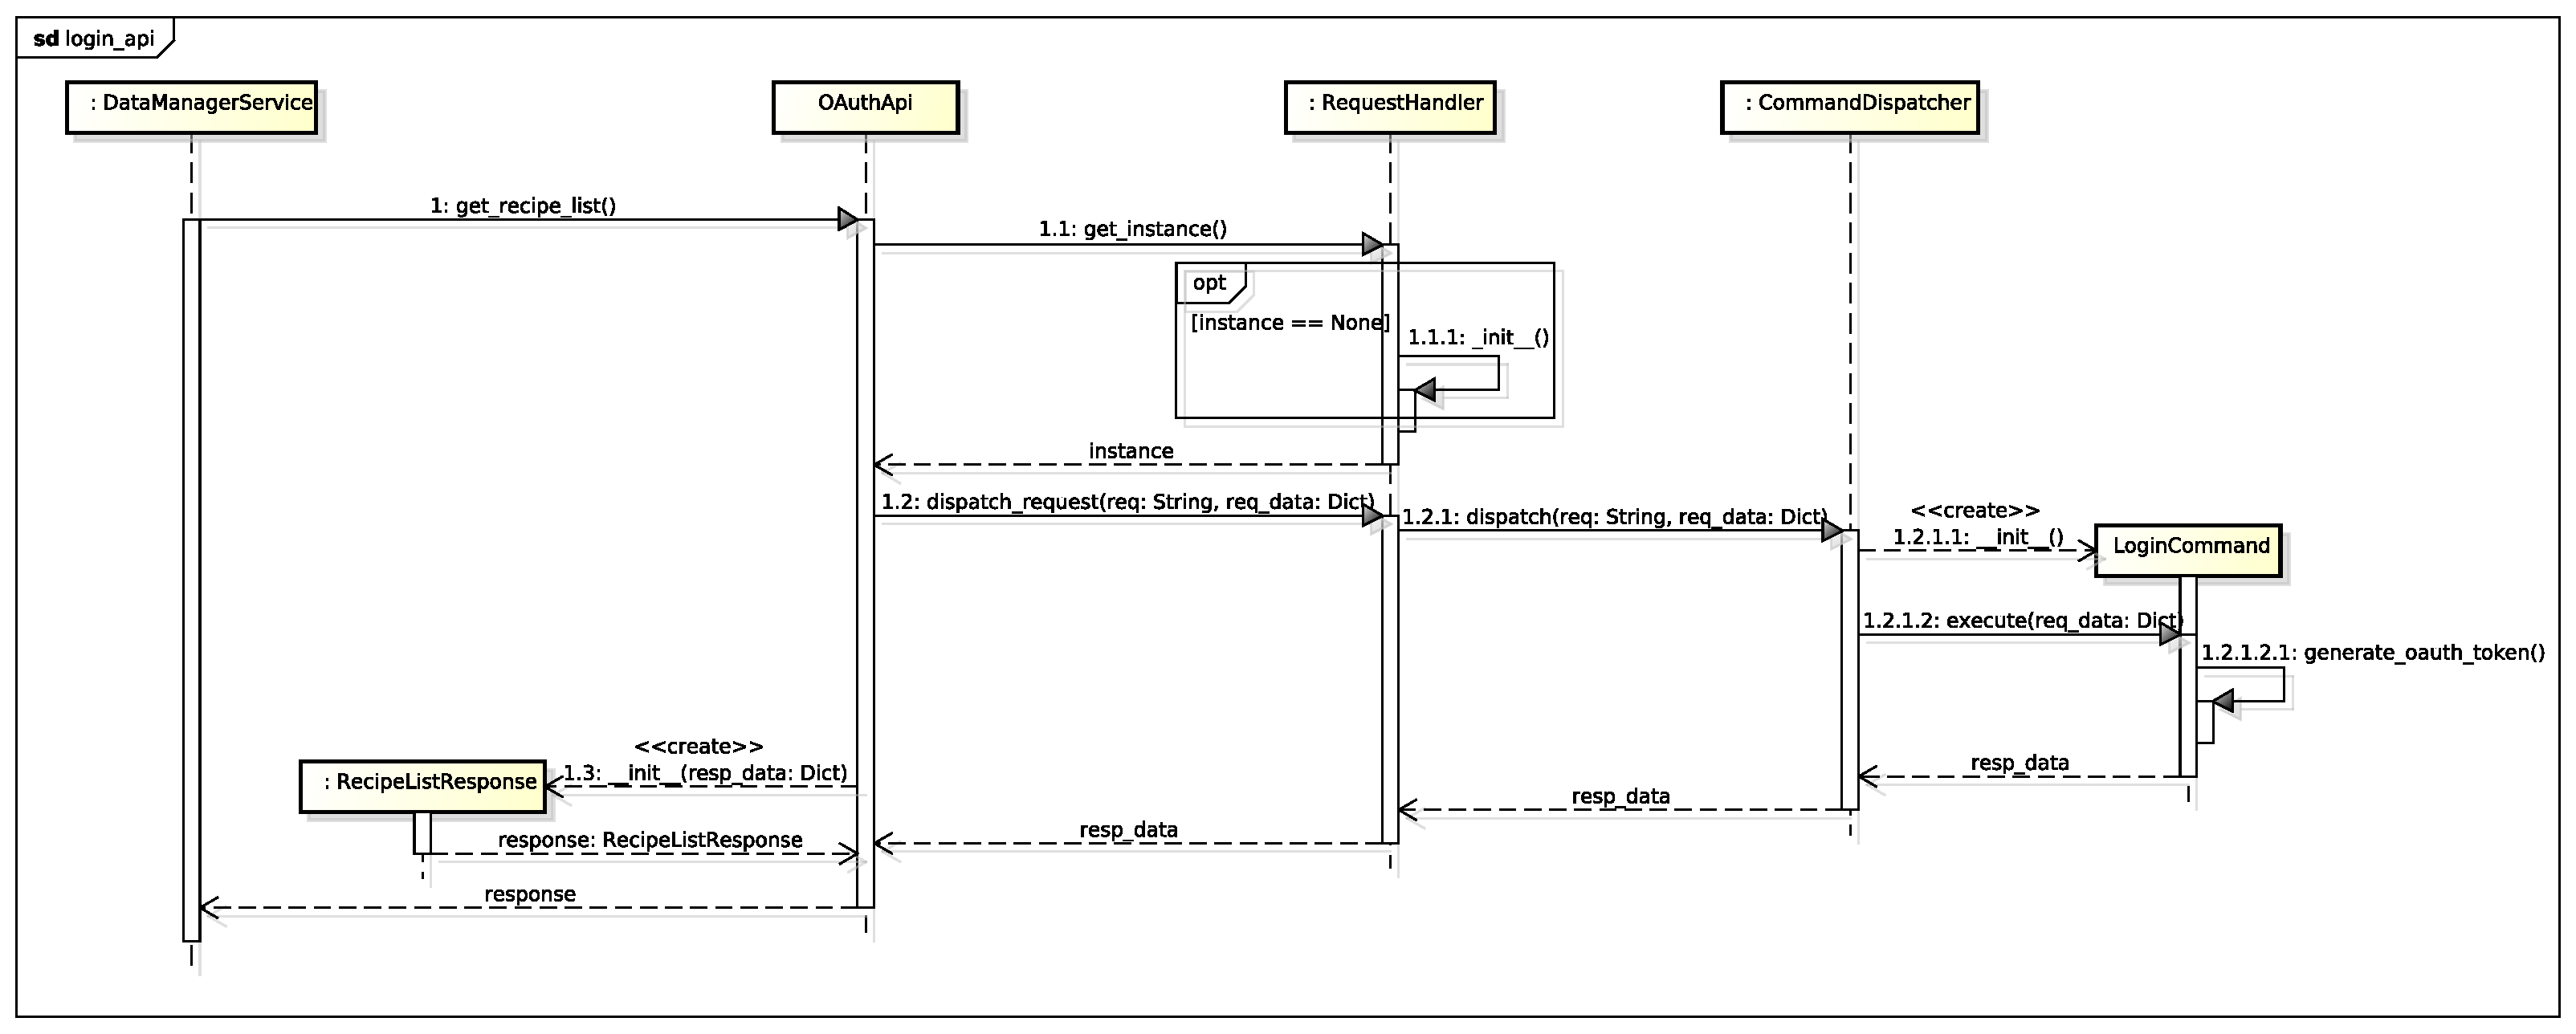
\includegraphics[angle=90, scale=0.4]{./images/sequence_diagram/login_api.pdf}}
		\caption{Diagramma di sequenza - Login API}
        \label{fig:login_api}
	\end{figure}


    \begin{itemize}
        \item \textbf{OAuthApi}: classe che riceve i dati di autenticazione dal client attraverso il metodo \texttt{login()} della classe \texttt{DataManagerService}. Si occupa di creare un'istanza della classe \texttt{RequestHandler} dopodiché richiama il processor passandogli il tipo di richiesta e il dizionario per soddisfare tale richiesta;
        \item \textbf{RequestHandler}: classe che rappresenta un singleton che viene istanziato dal metodo \texttt{get\_instance()} della classe \texttt{OAuthApi}. Attraverso il metodo \texttt{dispatch\_request()} riceve il tipo di richiesta e un dizionario contenente i dati per soddisfare tale richiesta;
        \item \textbf{CommandDispatcher}: classe che riceve il tipo di richiesta e il dizionario per soddisfare tale richiesta dalla classe \texttt{RequestHandler}. Si occupa di reindirizzare tale richiesta al command che si occupa di effettuare l'autenticazione;
        \item \textbf{LoginCommand}: classe che si occupa di soddisfare la richiesta di login ricevuta dal metodo \texttt{execute()} della classe \texttt{CommandDispatcher} ritornando i dati dell'utente che ha effettuato l'autenticazione e un access token generato tramite l'utilizzo del metodo \texttt{generate\_oauth\_token()};
        \item \textbf{UserResponse}: classe utilizzata dal metodo \texttt{login()} della classe \texttt{OAuthApi} per ritornare la risposta al client.
    \end{itemize}


	\subsubsection{Recipe List API} % (fold)
    \label{ssub:recipe_list_api}
    Il diagramma alla figura~\ref{fig:recipe_list} descrive il funzionamento del servizio REST offerto dal sistema e utile ad ottenere la lista di tutte le Recipe presenti nel sistema. Il client tramite il metodo \texttt{get\_recipe\_list()} della classe \texttt{DataManagerService} utilizza il servizio REST definito nella classe \texttt{MetricApi}. \newline

    \begin{figure}[!htbp]
		\centering
			\centerline{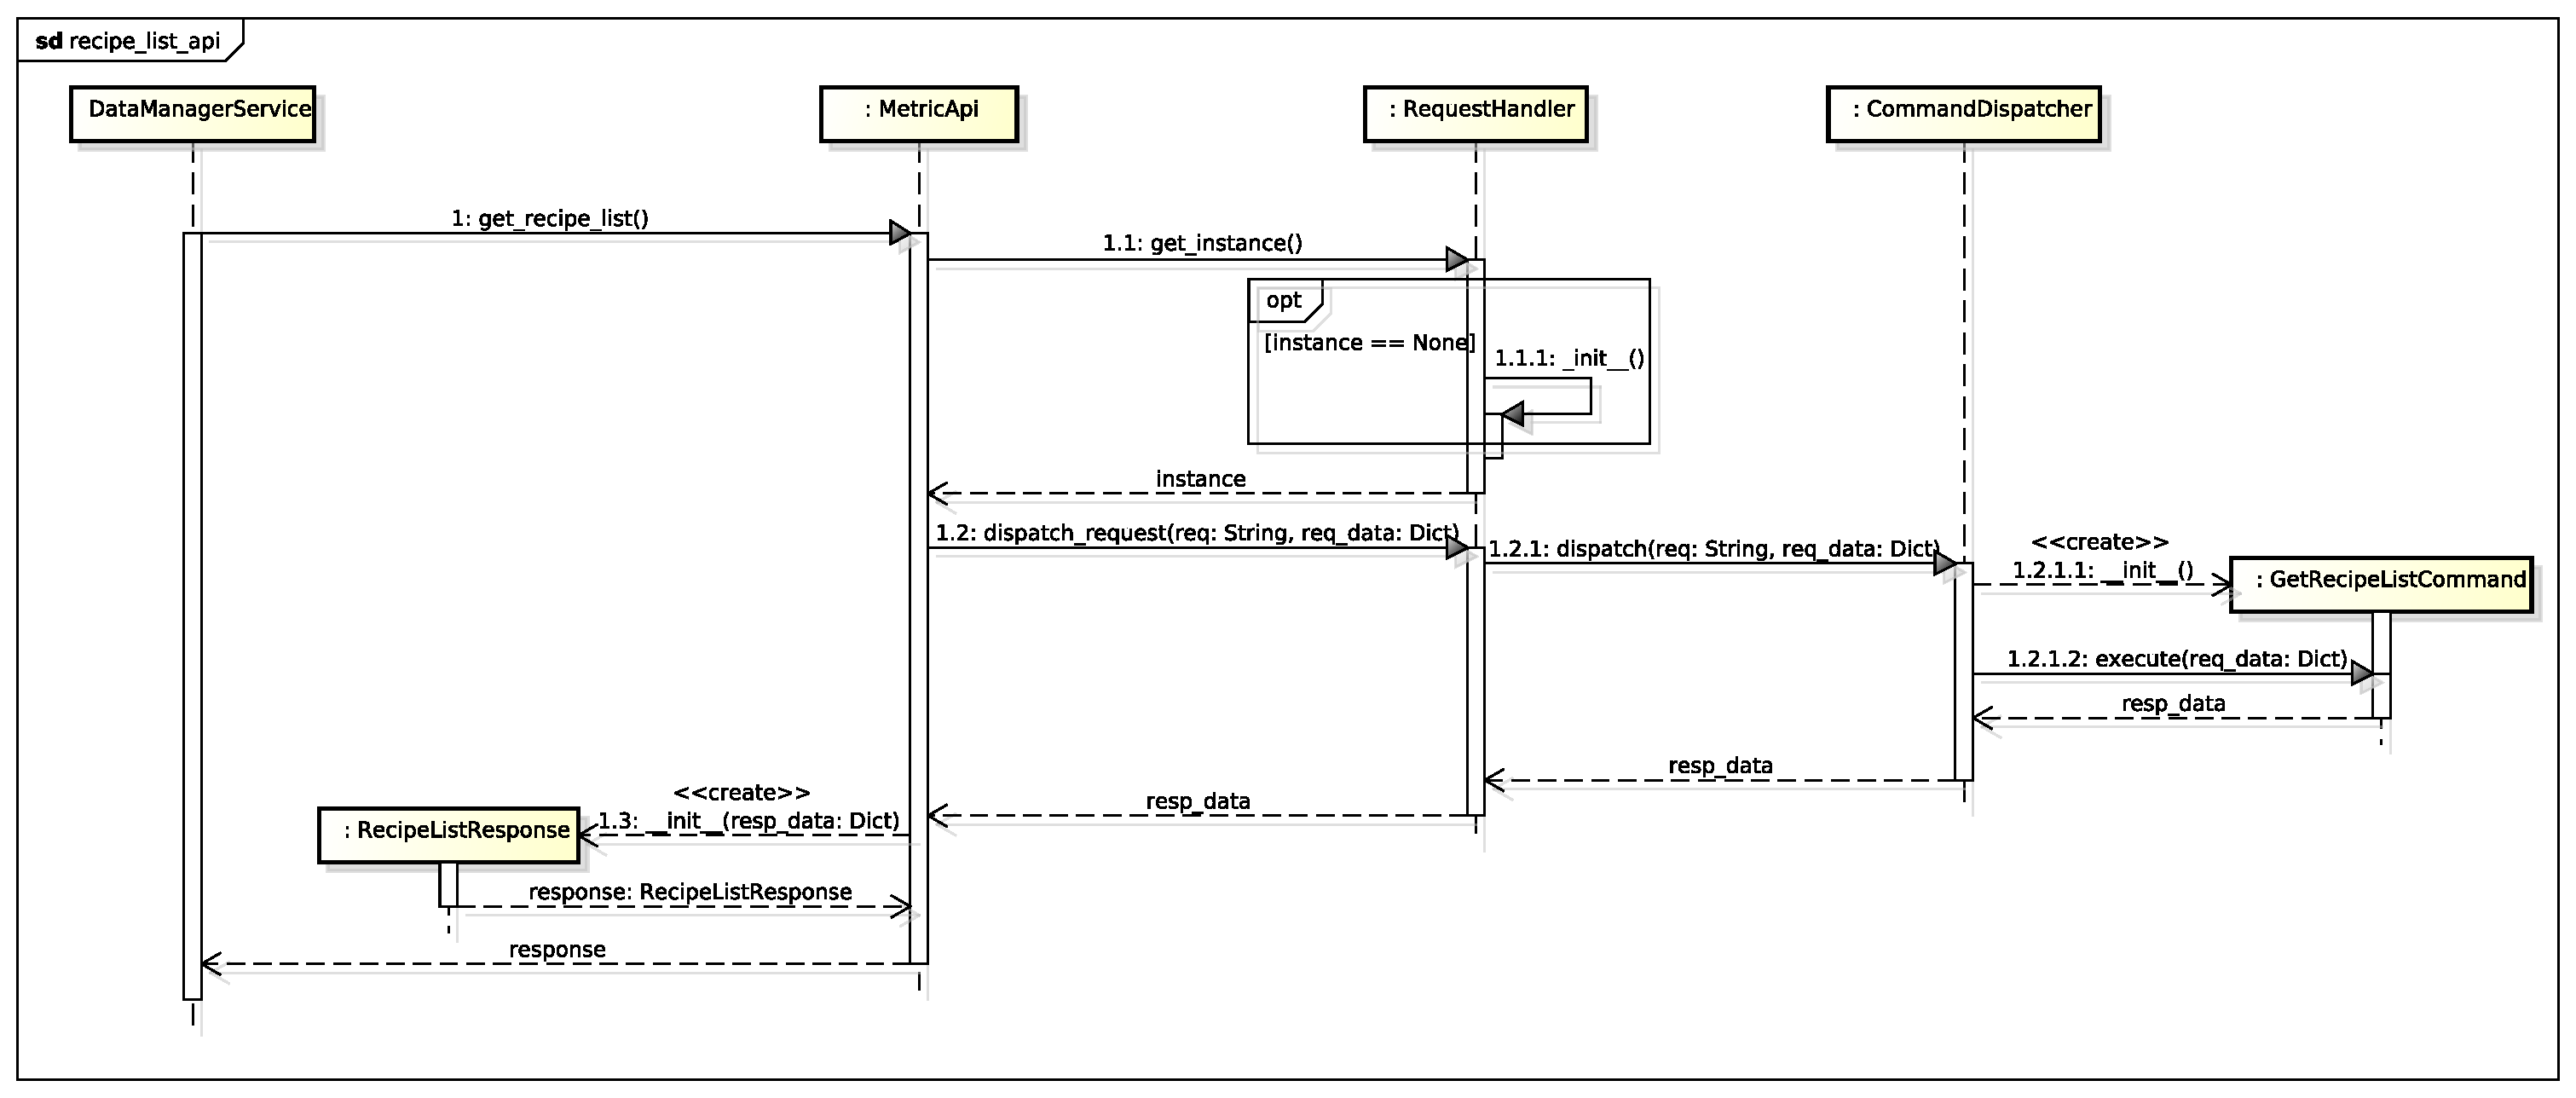
\includegraphics[angle=90, scale=0.4]{./images/sequence_diagram/recipe_list_api.pdf}}
		\caption{Diagramma di sequenza - Recipe List API}
        \label{fig:recipe_list}
	\end{figure}


    \begin{itemize}
        \item \textbf{MetricApi}: classe utilizzata dal client attraverso il metodo \texttt{get\_recipe\_list()} della classe \texttt{DataManagerService}. Si occupa di creare un'istanza della classe \texttt{RequestHandler} dopodiché richiama il processor passandogli il tipo di richiesta;
        \item \textbf{RequestHandler}: classe che rappresenta un singleton che viene istanziato dal metodo \texttt{get\_instance()} della classe \texttt{MetricApi}. Attraverso il metodo \texttt{dispatch\_request()} riceve il tipo di richiesta da soddisfare;
        \item \textbf{CommandDispatcher}: classe che riceve il tipo di richiesta da soddisfare dalla classe \texttt{RequestHandler}. Si occupa di reindirizzare tale richiesta al command che si occupa di prelevare tutte le Recipe dal sistema;
        \item \textbf{GetRecipeListCommand}: classe che si occupa di soddisfare la richiesta di prelievo di tutte le Recipe ricevuta dal metodo \texttt{execute()} della classe \texttt{CommandDispatcher} ritornando una lista contenente i dettagli di tutte le Recipe presenti nel sistema;
        \item \textbf{RecipeListResponse}: classe utilizzata dal metodo \texttt{get\_recipe\_list()} della classe \texttt{MetricApi} per ritornare la risposta al client.
    \end{itemize}
% section diagrammi_di_sequenza_server (end)